\documentclass[conference]{IEEEtran}

\usepackage{fontspec}
\IfFontExistsTF{Times New Roman}{\setmainfont{Times New Roman}}{\setmainfont{TeX Gyre Termes}}
\usepackage{cite}
\usepackage{amsmath,amssymb}
\usepackage{graphicx}
\usepackage{booktabs}
\usepackage{array}
\usepackage{xcolor}
\usepackage[hidelinks]{hyperref}
\expandafter\def\expandafter\UrlBreaks\expandafter{\UrlBreaks\do\-}
\graphicspath{{hinh/}}
\newcolumntype{L}[1]{>{\raggedright\arraybackslash}p{#1}}

\renewcommand{\topfraction}{0.85}
\renewcommand{\bottomfraction}{0.6}
\renewcommand{\textfraction}{0.12}
\renewcommand{\floatpagefraction}{0.75}
\renewcommand{\dbltopfraction}{0.85}
\renewcommand{\dblfloatpagefraction}{0.75}
\setcounter{topnumber}{3}
\setcounter{bottomnumber}{2}
\setcounter{totalnumber}{5}
\setcounter{dbltopnumber}{3}

\renewcommand{\abstractname}{Tóm tắt}
\renewcommand{\IEEEkeywordsname}{Từ khóa}
\renewcommand{\refname}{Tài liệu tham khảo}
\renewcommand{\figurename}{Hình}
\renewcommand{\tablename}{Bảng}

\begin{document}

\title{Kiểm chứng ngưỡng CVSS 8,0 của CSA và đề xuất công thức ưu tiên vá lỗ hổng kết hợp CVSS, EPSS và KEV}

\author{\IEEEauthorblockN{Trần Minh Vương (20252023M), Vũ Thành Huy (20252033M), Nguyễn Hoà Khiêm (20252031M)}
\IEEEauthorblockA{\textit{ĐẠI HỌC BÁCH KHOA HÀ NỘI}\\
\textit{TRƯỜNG CÔNG NGHỆ THÔNG TIN VÀ TRUYỀN THÔNG}}
}

\maketitle

\begin{abstract}
Báo cáo của Cloud Security Alliance (CSA) ngày 02/04/2026 khuyến nghị vá trong 48 giờ các lỗ hổng có CVSS trên
8,0 ảnh hưởng tới hệ thống phơi ra Internet. Trên 240.409 lỗ hổng có CVSS 3.x, với danh mục KEV của CISA làm căn
cứ, quy tắc này vá thừa ở mọi cách đọc: chỉ 1,3\% đến 1,5\% lỗ hổng trong diện vá khẩn cấp bị khai thác; tỷ lệ bỏ
sót từ 21\% đến 44\% tùy cách đọc. Chúng tôi đề xuất điểm ưu tiên $S$ từ 0 đến 100, kết hợp CVSS, EPSS, KEV, hai
biến của Chỉ thị BOD 26-04 (tự động hóa khai thác, phơi ra Internet) và mức quan trọng của tài sản. Kiểm thử ngược
tại 11 ngày đánh giá, chỉ dùng thông tin có tại ngày đó, cho thấy nhóm $S \ge 70$ chỉ chiếm 0,8\% đến 1,4\% số lỗ
hổng nhưng hiệu quả gấp 16 đến 34 lần chọn ngẫu nhiên, trong khi quy tắc CSA chỉ gấp 1,7 đến 2,3 lần; khi vá cùng
số lượng nhỏ, $S$ bắt được nhiều gấp 2,7 đến 8,9 lần cách xếp theo CVSS. Từ kết quả này, chúng tôi đề xuất thang
điểm $S$ kèm hạn vá để thay cho ngưỡng CVSS cố định. Hạn chế: $S$ gần như ngang EPSS dùng riêng, gần như không cảnh
báo trước được lỗ hổng mới công bố, và ba biến tài sản, phơi ra Internet, tự động hóa chưa kiểm chứng được bằng dữ
liệu công khai.
\end{abstract}

\begin{IEEEkeywords}
CVSS, EPSS, CISA KEV, BOD 26-04, ưu tiên vá lỗ hổng, chính sách an ninh mạng
\end{IEEEkeywords}

% =====================================================================
\section{Giới thiệu}
% =====================================================================

Riêng năm 2025 có 45.387 lỗ hổng có điểm CVSS 3.x trong NVD~\cite{nvd}. Không tổ chức nào vá kịp tất cả, nên câu
hỏi của quản trị an ninh mạng là \emph{vá lỗ hổng nào trước}. Báo cáo của CSA~\cite{csa2026} cho rằng mô hình ngôn
ngữ lớn (LLM) đã rút ngắn thời gian từ khi công bố lỗ hổng đến khi có mã khai thác, và khuyến nghị vá trong 48 giờ
các lỗ hổng có CVSS trên 8,0 trên hệ thống phơi ra Internet. Quy tắc này dễ áp dụng nhưng dựa vào CVSS, vốn đo
\emph{mức nghiêm trọng} chứ không đo \emph{khả năng bị khai thác}~\cite{cvss31}. Allodi và Massacci~\cite{allodi2014}
đã chỉ ra vá theo CVSS cao gần như tương đương vá ngẫu nhiên; EPSS~\cite{jacobs2021,epss} dự đoán khả năng bị khai
thác; VMC~\cite{shimizu2026} lọc hai bước theo KEV, EPSS rồi CVSS.

Báo cáo trả lời hai câu hỏi. (CH1) Trên dữ liệu thực, quy tắc ngưỡng CVSS 8,0 vá thừa và bỏ sót bao nhiêu? (CH2)
Một công thức kết hợp nhiều nguồn có sắp thứ tự ưu tiên tốt hơn quy tắc đó không, khi chỉ dùng thông tin có tại
thời điểm ra quyết định? Đóng góp gồm: (i) định lượng quy tắc CSA trên 240.409 lỗ hổng; (ii) công thức $S$ tích hợp
CVSS, EPSS, KEV, hai biến của BOD 26-04 và hệ số tài sản; (iii) kiểm thử ngược $S$ so với quy tắc CSA tại 11 ngày
đánh giá; (iv) thang điểm và hạn vá thay cho ngưỡng CVSS cố định.

% =====================================================================
\section{Khuyến nghị của CSA và vấn đề}\label{sec:csa}
% =====================================================================

CSA viết: \emph{``Security teams should treat published CVEs affecting internet-exposed systems with CVSS scores
above 8.0 as requiring emergency patching timelines \ldots\ CSA recommends organizations target remediation within
48 hours''}. Chúng tôi diễn đạt thành quy tắc phân loại
\begin{equation}
\mathit{CVSS} > 8{,}0 \wedge \text{phơi ra Internet} \Longrightarrow \text{vá trong 48 giờ}
\label{eq:csa}
\end{equation}
rồi xét nhóm ``vá khẩn cấp'' chứa được bao nhiêu lỗ hổng thực sự bị khai thác. Bài báo không giải thích hay kiểm
chứng ngưỡng 8,0, dù chính bài báo khuyên khung ưu tiên phải \emph{``weight exploitability heavily''}.

Dữ liệu gồm 240.409 lỗ hổng có CVSS 3.x trong NVD (mã CVE từ 1999 đến 2025), trong đó 1.570 nằm trong danh mục
KEV~\cite{kev} (phiên bản 2026.10.08). KEV là danh mục lỗ hổng CISA xác nhận đã bị khai thác, được dùng làm căn cứ
đúng; đây là căn cứ thận trọng vì lỗ hổng ngoài KEV chưa chắc không bị khai thác.

Bảng~\ref{tab:nguong} cho kết quả. Trong 66.722 lỗ hổng phải vá khẩn cấp, chỉ 877 (1,31\%) nằm trong KEV: phải vá
76,1 lỗ hổng mới gặp một lỗ hổng bị khai thác, tức 65.845 / 66.722 = 98,69\% là vá thừa. Ngược lại, 693 / 1.570 =
44,14\% lỗ hổng KEV có CVSS dưới 8,0 bị bỏ qua. Đổi ngưỡng chỉ chuyển gánh nặng giữa vá thừa và bỏ sót: ngưỡng 7,0
bỏ sót 11,40\% nhưng phải vá 54,33\% số lỗ hổng; ngưỡng 9,0 bỏ sót 65,99\%.

\begin{table}[htbp]
\caption{Các ngưỡng CVSS, 240.409 lỗ hổng từ 1999 đến 2025}\label{tab:nguong}
\centering
\begin{tabular}{lccc}
\toprule
Ngưỡng & Phải vá & Bỏ sót KEV & Bị khai thác \\
 & & & trong nhóm vá \\
\midrule
CVSS $\ge 7{,}0$ & 54,33\% & 11,40\% & 1,06\% \\
CVSS $\ge 8{,}0$ (CSA) & 27,75\% & 44,14\% & 1,31\% \\
CVSS $\ge 9{,}0$ & 14,43\% & 65,99\% & 1,54\% \\
\bottomrule
\end{tabular}
\end{table}

Để công bằng với CSA, chúng tôi thử năm cách đọc khuyến nghị (Bảng~\ref{tab:donhay}): Q1 đọc ``above 8.0'' theo
nghĩa chặt; Q2 chỉ xét lỗ hổng khai thác được qua mạng (vector \texttt{AV:N}), xấp xỉ điều kiện phơi ra Internet; Q3
thêm lỗ hổng đã có mã khai thác minh chứng (PoC) trên Exploit-DB~\cite{exploitdb}, theo lời khuyên khác của CSA; Q4
kết hợp Q2 và Q3. Đọc sát hơn chỉ giảm phần bỏ sót, từ 44,14\% xuống 20,73\%. Phần vá thừa không đổi: ở mọi cách đọc,
chỉ 1,31\% đến 1,51\% lỗ hổng trong nhóm phải vá bị khai thác, tức phải vá 66 đến 76 lỗ hổng mới gặp một lỗ hổng bị
khai thác. Vấn đề nằm ở thước đo: CVSS không chứa thông tin về việc lỗ hổng có đang bị khai thác hay không.

\begin{table}[htbp]
\caption{Năm cách đọc quy tắc CSA, 1999 đến 2025; Q2 và Q4 chỉ xét 174.803 lỗ hổng có vector \texttt{AV:N}}\label{tab:donhay}
\centering
\footnotesize
\setlength{\tabcolsep}{3pt}
\begin{tabular}{lcccc}
\toprule
Cách đọc & Phải vá & Bỏ sót KEV & Bị khai thác & Vá cho 1 ca \\
\midrule
Q0. CVSS $\ge 8{,}0$ & 27,75\% & 44,14\% & 1,31\% & 76,1 \\
Q1. CVSS $> 8{,}0$ & 27,35\% & 44,71\% & 1,32\% & 75,8 \\
Q2. Q0, chỉ \texttt{AV:N} & 35,97\% & 26,25\% & 1,34\% & 74,6 \\
Q3. Q0 hoặc có PoC & 29,01\% & 33,12\% & 1,51\% & 66,4 \\
Q4. Q3, chỉ \texttt{AV:N} & 37,11\% & 20,73\% & 1,40\% & 71,6 \\
\bottomrule
\end{tabular}
\end{table}

% =====================================================================
\section{Công thức đề xuất}\label{sec:giaiphap}
% =====================================================================

\subsection{Cơ sở: Chỉ thị BOD 26-04}
Ngày 10/06/2026, hai tháng sau bài báo CSA, CISA ban hành Chỉ thị BOD 26-04~\cite{bod2604}, thu hồi BOD 22-01 và BOD
19-02, thay hạn vá chung bằng bốn câu hỏi có hoặc không cho từng lỗ hổng trên từng tài sản: tài sản có \emph{phơi ra
Internet}, lỗ hổng có \emph{trong KEV}, việc khai thác có \emph{tự động hóa được} (Automatable: cả bốn bước trinh
sát, chế tạo mã khai thác, phát tán, khai thác chạy được mà không cần người can thiệp~\cite{ssvcauto}), và khai
thác thành công thì chiếm toàn quyền hay một phần hệ thống. Tổ hợp câu trả lời cho hạn vá 3, 14, 60 ngày hoặc hoãn
đến lần nâng cấp kế tiếp. Hướng dẫn thực hiện ghi rõ các cơ quan không còn bị yêu cầu dùng CVSS để xếp ưu
tiên~\cite{bod2604ig}. CISA dẫn số liệu Verizon DBIR 2026: chỉ 26\% lỗ hổng trong KEV được khắc phục hoàn toàn trong
năm 2025, giảm từ 38\% năm trước~\cite{cisablog2026,dbir2026}.

BOD 26-04 đi ngược khuyến nghị dùng ngưỡng CVSS 8,0: đặt bằng chứng khai thác, khả năng tự động hóa và mức phơi ra
Internet vào trung tâm. Công thức của chúng tôi lấy ba biến đầu của chỉ thị, giữ CVSS thay cho biến tác động kỹ
thuật, thêm EPSS để có xác suất liên tục cho lỗ hổng chưa có bằng chứng khai thác, và thêm hệ số tài sản. Khác với
BOD 26-04 chỉ chia bậc, công thức cho điểm liên tục để sắp thứ tự trong từng bậc.

\subsection{Công thức điểm ưu tiên}
Với mỗi cặp (lỗ hổng, tài sản):
\begin{equation}
\begin{split}
S = AC \times \mathit{CVSS} \times \Big[\,&\mathit{KEV} \times \mathit{PE}\\
&+ (1-\mathit{KEV}) \times \big(\mathit{EA} \times \mathit{PE}\\
&+ (1-\mathit{EA}) \times \mathit{EPSS}^{0{,}3}\big)\,\Big] \times 10.
\end{split}
\label{eq:S}
\end{equation}
Bảng~\ref{tab:bien} mô tả các biến. Gọi biểu thức trong ngoặc vuông là \emph{bộ lọc mối đe dọa} $T \in [0, 1]$; khi đó
$S = 10 \times AC \times \mathit{CVSS} \times T \in [0, 100]$. Điểm càng cao càng phải vá sớm.

\begin{table*}[t]
\centering
\caption{Các biến của công thức $S$}\label{tab:bien}
\small
\begin{tabular}{L{1.2cm}L{6.0cm}L{5.2cm}L{3.5cm}}
\toprule
Biến & Ý nghĩa & Giá trị & Nguồn \\
\midrule
$AC$ & Mức quan trọng của tài sản (không phải chỉ số Attack Complexity của CVSS) & 1,0 hệ thống lõi; 0,8 máy chủ nội bộ; 0,5 máy trạm; 0,2 thiết bị thử nghiệm & CMDB của tổ chức \\
$\mathit{CVSS}$ & Mức nghiêm trọng kỹ thuật & 0 đến 10 & NVD \\
$\mathit{KEV}$ & Đã bị khai thác thực tế & 1 nếu có trong KEV tại thời điểm đánh giá & CISA KEV \\
$\mathit{EA}$ & Tự động hóa khai thác được (Automatable, BOD 26-04) & 1 nếu Yes, 0 nếu No & CISA Vulnrichment~\cite{vulnrichment} \\
$\mathit{PE}$ & Tài sản phơi ra Internet (Publicly Exposed, BOD 26-04) & 1 nếu truy cập được từ Internet & Công cụ quản lý bề mặt tấn công \\
$\mathit{EPSS}$ & Xác suất bị khai thác trong 30 ngày tới & 0 đến 1 & FIRST EPSS~\cite{epss} \\
\bottomrule
\end{tabular}
\end{table*}

\subsection{Cắt nghĩa công thức}
Vì $\mathit{KEV}$, $\mathit{EA}$, $\mathit{PE}$ chỉ nhận 0 hoặc 1, bộ lọc $T$ tự rẽ năm nhánh mà không cần câu lệnh
điều kiện (Bảng~\ref{tab:nhanh}).

\begin{table}[t]
\centering
\caption{Năm trường hợp của bộ lọc mối đe dọa $T$}\label{tab:nhanh}
\footnotesize
\setlength{\tabcolsep}{3pt}
\begin{tabular}{cccc L{4.1cm}}
\toprule
$\mathit{KEV}$ & $\mathit{EA}$ & $\mathit{PE}$ & $T$ & Ý nghĩa \\
\midrule
1 & 0, 1 & 1 & 1 & Đã bị khai thác, phơi ra Internet: cao nhất \\
1 & 0, 1 & 0 & 0 & Đã bị khai thác, trong mạng nội bộ: xử lý bằng quy tắc chính sách \\
0 & 1 & 1 & 1 & Tự động hóa được, phơi ra Internet: cao nhất, không chờ EPSS \\
0 & 1 & 0 & 0 & Tự động hóa được nhưng công cụ quét từ Internet không thấy \\
0 & 0 & 0, 1 & $\mathit{EPSS}^{0{,}3}$ & Không tự động hóa được: tăng dần theo EPSS \\
\bottomrule
\end{tabular}
\end{table}

\begin{itemize}
\item \textbf{Nhánh KEV và nhánh tự động hóa nhân với $\mathit{PE}$.} Lỗ hổng đã bị khai thác hoặc có thể bị quét và
tấn công hàng loạt chỉ là mối nguy cao nhất khi kẻ tấn công từ Internet tiếp cận được tài sản; khi đó $T = 1$ và
$S = 10 \times AC \times \mathit{CVSS}$. Nhánh tự động hóa đúng là kịch bản CSA lo ngại khi LLM tự động hóa việc tạo
mã khai thác.
\item \textbf{Nhánh EPSS không nhân với $\mathit{PE}$.} EPSS học từ tấn công toàn cầu, gồm cả các con đường không đi
trực tiếp từ Internet như thư lừa đảo, mối đe dọa nội bộ, VPN. Nhân $\mathit{PE}$ sẽ đưa mọi lỗ hổng trong mạng nội
bộ về 0, trong khi kẻ tấn công vẫn vào được mạng nội bộ qua máy nhân viên.
\item \textbf{Số mũ 0,3.} Phần lớn EPSS rất nhỏ; nhân thẳng sẽ làm điểm dồn về 0. Số mũ 0,3 nén thang mà giữ thứ tự:
$0{,}001 \mapsto 0{,}13$, $0{,}01 \mapsto 0{,}25$, $0{,}1 \mapsto 0{,}50$. Ở nhánh EPSS, xếp theo $S$ trùng với xếp
theo $\mathit{EPSS} \times \mathit{CVSS}^{3{,}33}$.
\item \textbf{Hệ số $AC$.} Cùng một lỗ hổng trên máy chủ thanh toán ($AC = 1$) phải vá trước khi nằm trên máy thử
nghiệm ($AC = 0{,}2$). $AC$ chỉ đo mức quan trọng nghiệp vụ; mức phơi ra Internet do $\mathit{PE}$ đo riêng.
\end{itemize}

\subsection{Quy tắc chính sách đi kèm}
\begin{itemize}
\item \textbf{Lỗ hổng có $T = 1$ luôn thuộc nhóm vá khẩn cấp.} Ở nhánh này $S = 10 \times AC \times \mathit{CVSS}$,
nên một lỗ hổng đã bị khai thác có CVSS 6,5 chỉ được 65 điểm, dưới ngưỡng 70. Ngày 30/06/2025, 160 / 1.371 = 11,67\%
lỗ hổng trong KEV rơi vào trường hợp này.
\item \textbf{Lỗ hổng trong KEV trên tài sản nội bộ vẫn có hạn vá tối đa} theo Bảng 1 của BOD 26-04 (14 ngày, hoặc
3 ngày kèm điều tra xâm nhập), dù $S = 0$, vì kẻ tấn công đã vào mạng nội bộ thường dùng chính các lỗ hổng này để
di chuyển ngang.
\end{itemize}

\subsection{Ví dụ so với quy tắc CSA}
Bảng~\ref{tab:vidu} so sánh trên bảy lỗ hổng giả định. Quy tắc CSA chọn A và D, bỏ qua B (EPSS 0,90) và C (đã bị
khai thác). Công thức đưa D lên đầu vì tự động hóa được và phơi ra Internet (nếu $\mathit{EA} = 0$, D chỉ được 45,1),
xếp B thứ hai, đưa C vào nhóm vá khẩn cấp nhờ quy tắc $T = 1$, và hạ A xuống 12,3 vì gần như không có tín hiệu khai
thác. Trong mạng nội bộ, E và F về 0 (F vẫn có hạn vá tối đa), còn G vẫn được 54,4 nhờ EPSS.

\begin{table}[t]
\centering
\caption{Ví dụ điểm $S$ với $AC = 1$ (số liệu giả định)}\label{tab:vidu}
\footnotesize
\setlength{\tabcolsep}{3pt}
\begin{tabular}{ccccccrl}
\toprule
 & CVSS & EPSS & KEV & EA & PE & $S$ & Quy tắc CSA \\
\midrule
A & 9,8 & 0,001 & 0 & 0 & 1 & 12,3 & vá 48 giờ \\
B & 7,5 & 0,90 & 0 & 0 & 1 & 72,7 & bỏ qua \\
C & 6,5 & không xét & 1 & không xét & 1 & 65,0 & bỏ qua \\
D & 9,0 & 0,10 & 0 & 1 & 1 & 90,0 & vá 48 giờ \\
E & 9,0 & 0,10 & 0 & 1 & 0 & 0,0 & ngoài phạm vi \\
F & 8,8 & không xét & 1 & không xét & 0 & 0,0 & ngoài phạm vi \\
G & 7,8 & 0,30 & 0 & 0 & 0 & 54,4 & ngoài phạm vi \\
\bottomrule
\end{tabular}
\end{table}

\subsection{Dạng rút gọn được kiểm chứng}
Trên tài sản phơi ra Internet ($\mathit{PE} = 1$, đúng phạm vi của CSA) và khi chưa dùng biến tự động hóa
($\mathit{EA} = 0$), công thức~\eqref{eq:S} rút gọn thành
\begin{equation}
S_0 = AC \times \mathit{CVSS} \times \left[\mathit{KEV} + (1-\mathit{KEV}) \times \mathit{EPSS}^{0{,}3}\right] \times 10.
\label{eq:S0}
\end{equation}
Các thực nghiệm kiểm chứng dạng~\eqref{eq:S0} với $AC = 1$. Nhánh KEV không cần chứng minh vì lỗ hổng đã bị khai
thác; phần cần chứng minh là nhánh chưa có trong KEV. $\mathit{PE}$ và $AC$ cần dữ liệu tài sản của tổ chức;
$\mathit{EA}$ có trong Vulnrichment nhưng chỉ phủ khoảng 45,8\% số CVE theo ước tính của Securin~\cite{securin2026},
và có thể được chấm sau khi lỗ hổng đã bị khai thác.

% =====================================================================
\section{Cách so sánh với quy tắc CSA}\label{sec:trienkhai}
% =====================================================================

\textbf{Kiểm thử ngược.} Đứng ở ngày $T$ trong quá khứ, lấy các lỗ hổng đã công bố và chưa có trong KEV, tính $S$
bằng EPSS lịch sử đúng ngày $T$, rồi gắn nhãn bị khai thác nếu lỗ hổng vào KEV trong 365 ngày sau $T$. Phải dùng EPSS
lịch sử vì EPSS hiện tại của lỗ hổng đã bị khai thác thường cao \emph{do} việc khai thác đã xảy ra. Thực nghiệm chạy
tại ba ngày 31/12/2023, 31/12/2024, 30/06/2025, và lặp lại tại 11 ngày cuối quý từ 31/03/2023 đến 30/09/2025.

\textbf{Thước đo.} \emph{Hiệu suất} là tỷ lệ lỗ hổng bị khai thác bắt được chia cho tỷ lệ khối lượng phải vá, tức
cách chọn đó tốt gấp bao nhiêu lần chọn ngẫu nhiên. Khi so hai cách xếp hạng, cố định \emph{cùng khối lượng vá}
(1\%, 5\% hoặc bằng khối lượng của quy tắc CSA); khoảng tin cậy 95\% tính bằng bootstrap 1.000 lần.

\textbf{Giả thuyết đặt trước H1.} Lỗ hổng 2023 đến 2025 chia đợt theo tháng công bố, ngày quyết định là cuối tháng,
nhãn là vào KEV trong 180 ngày; 2024 và 2025 là năm kiểm thử. H1: ở cùng khối lượng vá với quy tắc CSA, $S$ bắt được
nhiều hơn CVSS, đạt nếu khoảng tin cậy 95\% nằm trên 0.

\textbf{Tình huống điển hình.} Chọn theo tiêu chí đặt trước và báo cáo cả số trường hợp không đạt. Toàn bộ dữ liệu
công khai; mã nguồn chỉ đọc siêu dữ liệu lỗ hổng, không tạo mã khai thác hay quét hệ thống nào.

% =====================================================================
\section{Kết quả: công thức S so với quy tắc CSA}\label{sec:ketqua}
% =====================================================================

\subsection{Điểm S phân biệt được lỗ hổng sắp bị khai thác}
Ngày 30/06/2025 có 209.623 lỗ hổng chưa có trong KEV, chỉ 91 (0,043\%) vào KEV trong 12 tháng sau. Tỷ lệ vào KEV
tăng đều theo mức điểm (Bảng~\ref{tab:mucS}): mức từ 70 có tỷ lệ 1,21\%, gấp 28 lần trung bình; mức dưới 10 chỉ
0,011\%. Ba mức 70 đến 79, 80 đến 89, 90 đến 100 có tỷ lệ gần như nhau (1,16\%, 1,29\%, 1,22\%), nên ngưỡng vá khẩn
cấp được đặt ở 70.

\begin{table}[htbp]
\caption{Tỷ lệ vào KEV trong 12 tháng theo mức $S$, ngày 30/06/2025}\label{tab:mucS}
\centering
\footnotesize
\setlength{\tabcolsep}{4pt}
\begin{tabular}{lrrrr}
\toprule
Mức $S$ & Số lỗ hổng & Vào KEV & Tỷ lệ & Gấp TB \\
\midrule
70 đến 100 & 2.803 & 34 & 1,21\% & 28 \\
50 đến 69 & 4.065 & 12 & 0,30\% & 7 \\
30 đến 49 & 11.310 & 11 & 0,097\% & 2,2 \\
10 đến 29 & 90.626 & 23 & 0,025\% & 0,6 \\
0 đến 9 & 100.819 & 11 & 0,011\% & 0,3 \\
\midrule
Tổng & 209.623 & 91 & 0,043\% & 1,0 \\
\bottomrule
\end{tabular}
\end{table}

\subsection{Ngưỡng S từ 70 so với quy tắc CSA}
Bảng~\ref{tab:khancap} đặt hai cách cạnh nhau. Ngày 30/06/2025, vá mọi lỗ hổng có $S \ge 70$ là vá 2.803 lỗ hổng
(1,34\%) và bắt được 34/91; quy tắc CSA vá 58.133 lỗ hổng (27,73\%) và bắt 54/91. Quy tắc CSA bắt nhiều hơn vì vá
nhiều gấp khoảng 20 lần: phải vá 1.076 lỗ hổng cho mỗi lỗ hổng bắt được, so với 82 của $S \ge 70$. Tính theo hiệu
suất, $S \ge 70$ gấp 22,6 đến 27,9 lần chọn ngẫu nhiên, quy tắc CSA chỉ 2,1 lần.

\begin{table}[htbp]
\caption{Ngưỡng $S \ge 70$ và quy tắc CSA trên phần chưa có trong KEV. HS: hiệu suất, số lần so với chọn ngẫu
nhiên; khẩn cấp: nhóm $S \ge 70$ cộng mọi lỗ hổng đã có trong KEV}\label{tab:khancap}
\centering
\footnotesize
\setlength{\tabcolsep}{3pt}
\begin{tabular}{lccccc}
\toprule
 & \multicolumn{3}{c}{Ngưỡng $S \ge 70$} & \multicolumn{2}{c}{Quy tắc CSA} \\
\cmidrule(lr){2-4}\cmidrule(lr){5-6}
Ngày & Bắt được & HS & Khẩn cấp & Khối lượng & HS \\
\midrule
31/12/2023 & 14/61 & 22,6 & 1,72\% & 28,98\% & 2,1 \\
31/12/2024 & 16/80 & 25,5 & 1,44\% & 28,20\% & 2,1 \\
30/06/2025 & 34/91 & 27,9 & 1,98\% & 27,73\% & 2,1 \\
\bottomrule
\end{tabular}
\end{table}

Kết quả ổn định qua 11 ngày cuối quý (776 lượt lỗ hổng vào KEV): nhóm $S \ge 70$ chỉ chiếm 0,78\% đến 1,40\% số lỗ
hổng chưa có trong KEV nhưng hiệu suất gấp 15,9 đến 34,2 lần; quy tắc CSA ở mọi cách đọc chỉ 1,7 đến 2,3 lần. Tính
cả lỗ hổng đã có trong KEV, nhóm vá khẩn cấp theo $S$ chỉ chiếm 1,44\% đến 1,98\% số lỗ hổng, thay vì khoảng 28\%
như quy tắc CSA. Khi vá cùng khối lượng với từng cách đọc Q0 đến Q4 tại ba ngày, $S$ bắt được bằng hoặc nhiều hơn
quy tắc ở 13/15 trường hợp; hai trường hợp ngược lại đều ở năm 2024 với cách đọc có PoC (Q3: 55 so với 49; Q4: 51
so với 46), cho thấy PoC công khai là tín hiệu có giá trị mà $S$ chưa dùng.

\begin{figure}[t]
\centering
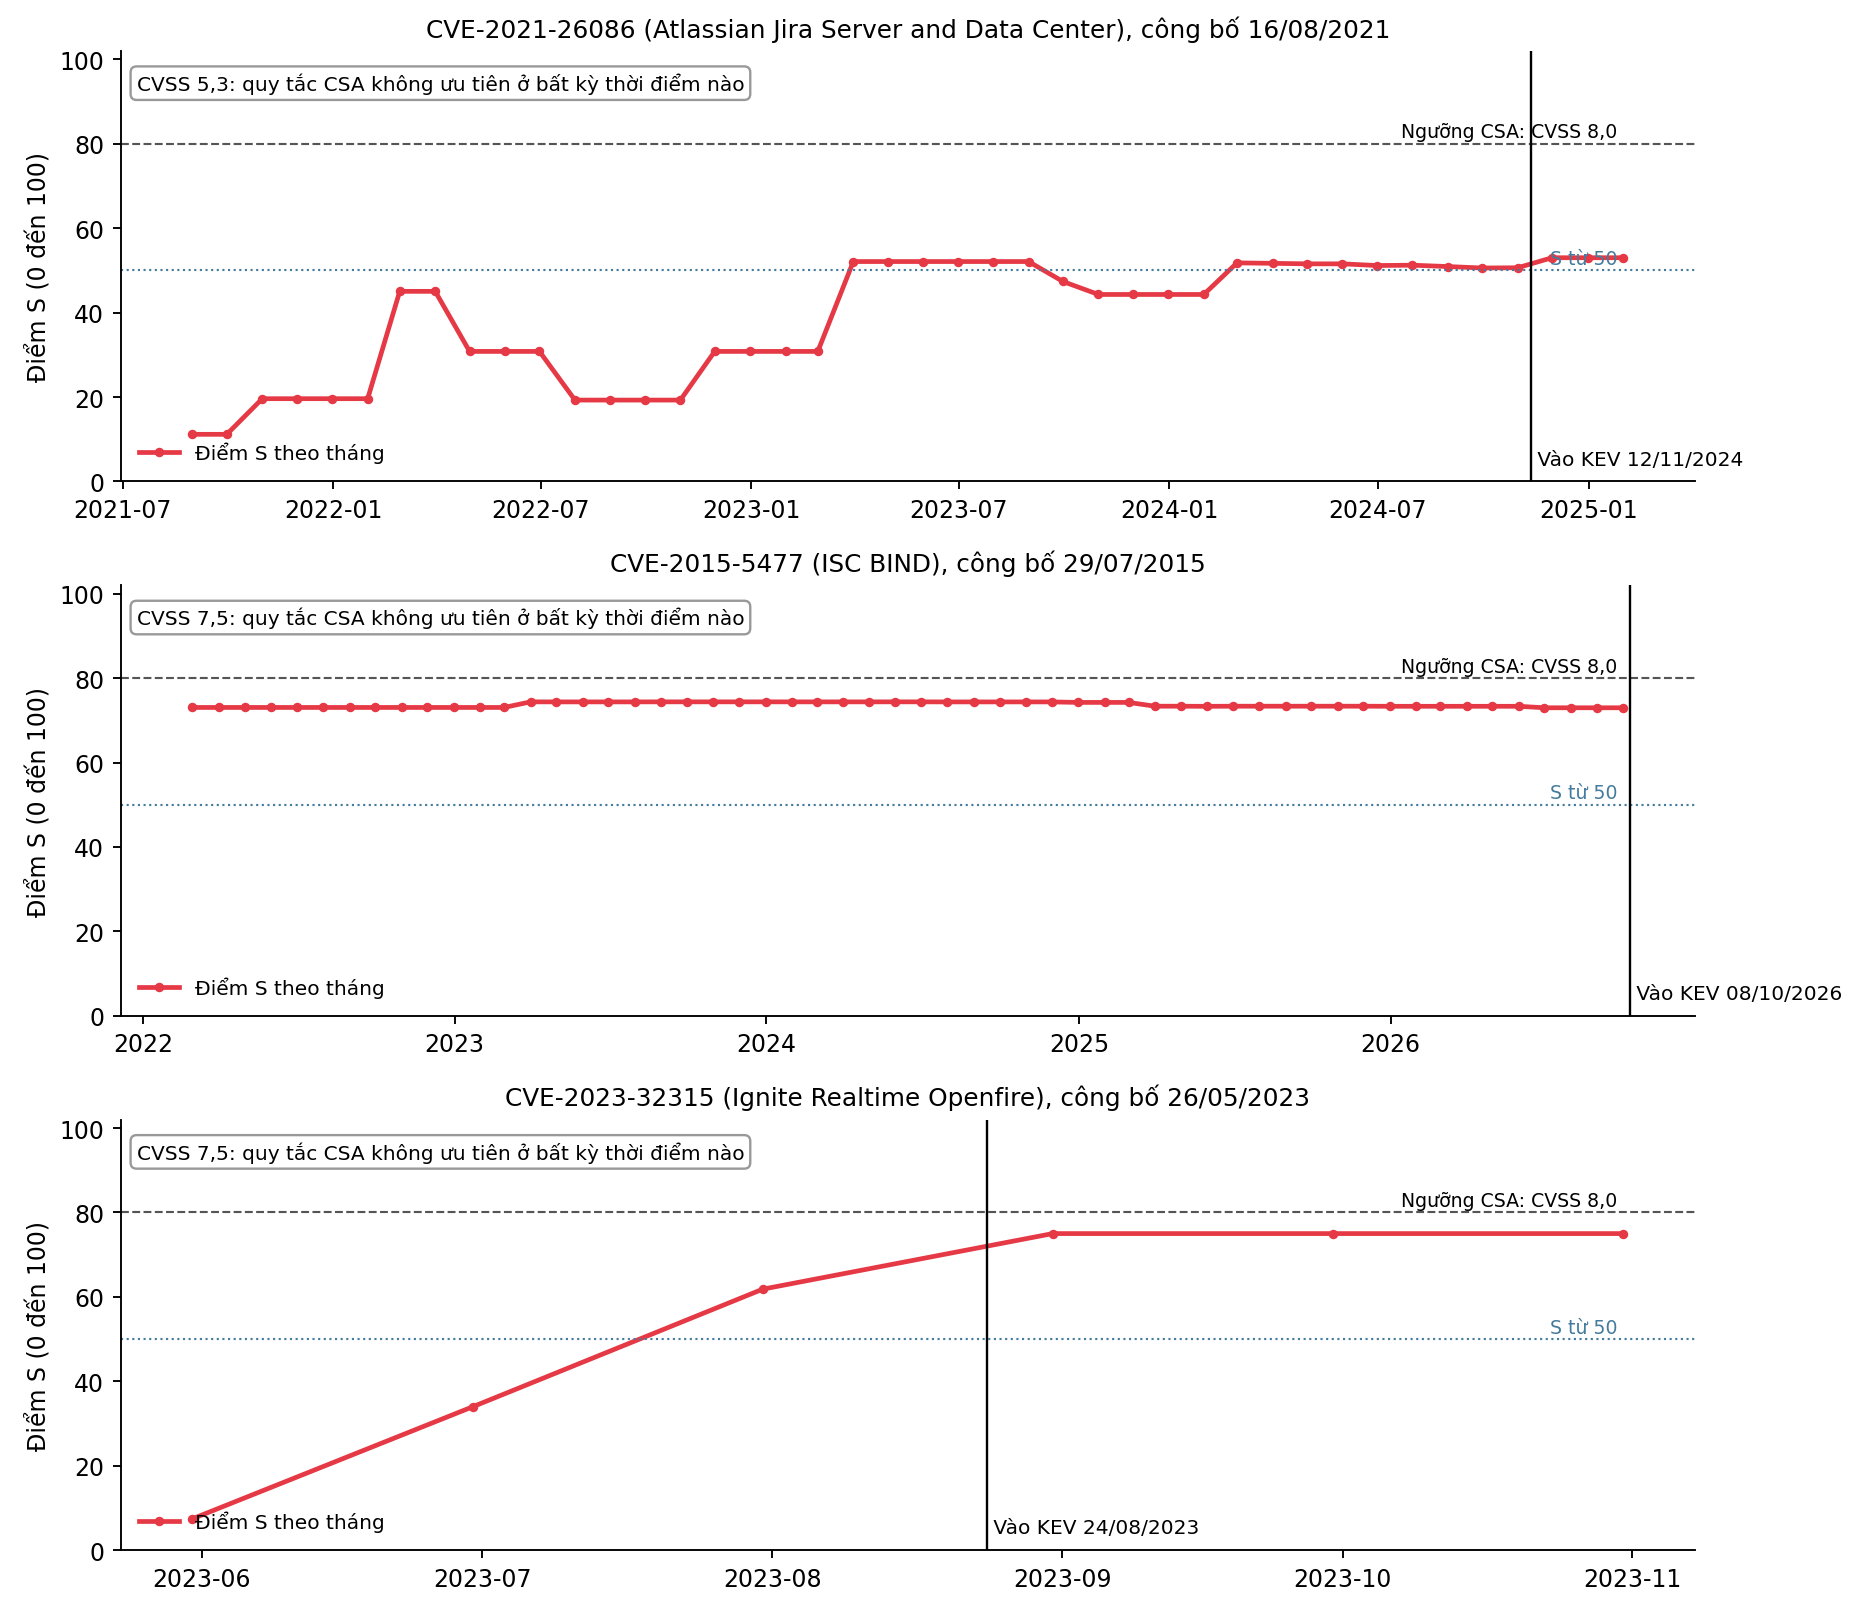
\includegraphics[width=\columnwidth]{tinh_huong_lich_su_diem.png}
\caption{Điểm $S$ theo tháng của ba tình huống. Đường nét đứt ở 80 ứng với ngưỡng CVSS 8,0 (nhân 10), đường chấm ở
50 là ngưỡng ưu tiên cao, đường thẳng đứng là ngày vào KEV; cả ba có CVSS dưới 8,0 nên quy tắc CSA không ưu tiên ở
bất kỳ thời điểm nào.}\label{fig:tinhhuong}
\end{figure}

\subsection{Cùng khối lượng vá}
Bảng~\ref{tab:cungkl} cố định số lỗ hổng được vá. Khi vá 1\% hoặc 5\%, $S$ bắt được nhiều gấp 2,7 đến 8,9 lần xếp
theo CVSS ở cả ba ngày, khoảng tin cậy 95\% của chênh lệch đều trên 0. Qua 11 ngày, $S$ không kém CVSS ở bất kỳ ngày
nào và ở bất kỳ khối lượng vá nào. Cột EPSS cho thấy phần lớn khả năng dự đoán của $S$ đến từ EPSS: hai cách gần như
ngang nhau, chênh lệch đổi chiều theo ngày. Hình~\ref{fig:ondinh} cho thấy khi vá 5\%, đường của $S$ nằm trên đường
của CVSS ở cả 11 ngày.

\begin{figure}[t]
\centering
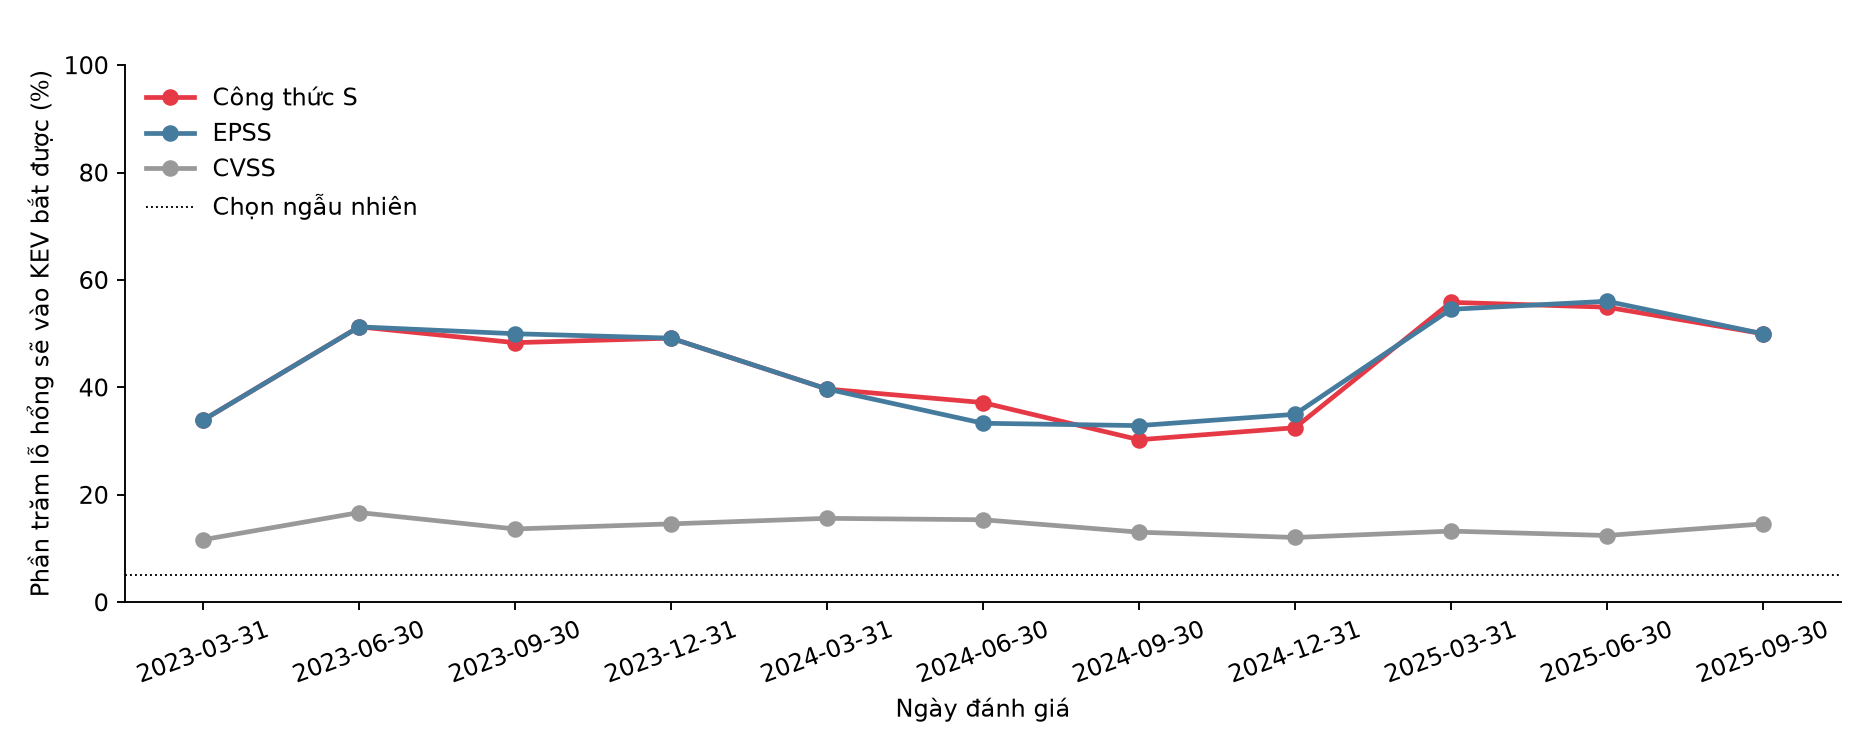
\includegraphics[width=\columnwidth]{nhieu_ngay_va_5.png}
\caption{Vá 5\% số lỗ hổng chưa có trong KEV tại 11 ngày đánh giá: phần trăm lỗ hổng vào KEV trong 12 tháng sau mà
mỗi cách bắt được. Đường chấm là chọn ngẫu nhiên.}\label{fig:ondinh}
\end{figure}

\begin{table}[htbp]
\caption{Số lỗ hổng vào KEV trong 12 tháng bắt được khi vá cùng số lượng}\label{tab:cungkl}
\centering
\footnotesize
\setlength{\tabcolsep}{3.5pt}
\begin{tabular}{llrccc}
\toprule
Ngày & Vá & Số vá & CVSS & EPSS & $S$ \\
\midrule
31/12/2023 & 1\%    & 1.473  & 2,0/61  & 14/61 & 14/61 \\
           & 5\%    & 7.365  & 8,9/61  & 30/61 & 30/61 \\
           & như CSA & 42.685 & 38/61  & 49/61 & 51/61 \\
31/12/2024 & 1\%    & 1.867  & 2,0/80  & 18/80 & 18/80 \\
           & 5\%    & 9.337  & 9,7/80  & 28/80 & 26/80 \\
           & như CSA & 52.662 & 48/80  & 45/80 & 48/80 \\
30/06/2025 & 1\%    & 2.096  & 4,8/91  & 30/91 & 25/91 \\
           & 5\%    & 10.481 & 11,3/91 & 51/91 & 50/91 \\
           & như CSA & 58.133 & 54/91  & 65/91 & 65/91 \\
\bottomrule
\end{tabular}
\end{table}

\textbf{H1 chưa đạt.} Ở đúng khối lượng vá của quy tắc CSA, gộp 2024 và 2025, $S$ bắt được nhiều hơn CVSS 6,0 ca,
khoảng tin cậy 95\% $[-2{,}0;\ +15{,}0]$ có chứa 0. Khi vá ít hơn (phân tích khám phá), chênh lệch có ý nghĩa thống
kê: $+12{,}6$ ca $[+3{,}9;\ +21{,}8]$ khi vá 1\%, $+18{,}2$ ca $[+8{,}3;\ +28{,}5]$ khi vá 5\%. Lợi thế của $S$ vì
vậy rõ nhất khi nguồn lực vá có hạn, đúng tình huống của hạn 48 giờ.

\begin{table*}[t]
\centering
\caption{Thang điểm $S$ và hạn vá khuyến nghị. Tỷ lệ vào KEV lấy từ Bảng~\ref{tab:mucS}}\label{tab:thangdiem}
\small
\begin{tabular}{L{3.6cm}L{3.0cm}L{6.6cm}L{3.0cm}}
\toprule
Điều kiện hoặc mức $S$ & Phân loại & Ý nghĩa & Hạn vá \\
\midrule
$\mathit{KEV} = 1$, $\mathit{PE} = 1$ & \textbf{Khẩn cấp, đã bị khai thác} & Đã bị khai thác và tài sản phơi ra Internet & \textbf{3 ngày}, kèm điều tra xâm nhập \\
$\mathit{KEV} = 0$, $\mathit{EA} = 1$, $\mathit{PE} = 1$ & \textbf{Khẩn cấp, tự động hóa được} & Có thể bị quét và tấn công tự động trên diện rộng & \textbf{3 ngày} \\
$\mathit{KEV} = 1$, $\mathit{PE} = 0$ ($S = 0$) & Đã bị khai thác, tài sản nội bộ & Kẻ tấn công trong mạng có thể dùng để di chuyển ngang & \textbf{14 ngày}; 3 ngày nếu tự động hóa được và chiếm toàn quyền \\
$\mathit{KEV} = 0$, $\mathit{EA} = 1$, $\mathit{PE} = 0$ ($S = 0$) & Tự động hóa được, tài sản nội bộ & Theo Bảng 1 của BOD 26-04 & \textbf{60 ngày} \\
\midrule
70 đến 100 & \textbf{Nghiêm trọng} & Tỷ lệ vào KEV 1,21\%, gấp 28 lần trung bình. Cần CVSS 9,8 với EPSS từ khoảng 0,33. CVSS dưới 7,0 không thể vào mức này & \textbf{7 ngày} \\
50 đến 69 & \textbf{Cao} & 0,30\%, gấp 7 lần trung bình & \textbf{14 ngày} \\
30 đến 49 & \textbf{Trung bình} & 0,097\%, gấp 2,2 lần trung bình & \textbf{30 ngày} \\
10 đến 29 & \textbf{Thấp} & 0,025\%; phần lớn lỗ hổng CVSS cao nhưng EPSS nhỏ nằm ở đây & \textbf{60 ngày} \\
0 đến 9 & \textbf{Rất thấp} & 0,011\%, gần như chưa có tín hiệu khai thác & Lần nâng cấp kế tiếp \\
\bottomrule
\end{tabular}
\end{table*}

\begin{table*}[t]
\centering
\caption{Danh sách đầy đủ 24 lỗ hổng mà công thức bắt trước còn quy tắc CSA bỏ qua: CVSS dưới 8,0 và $S \ge 50$ tại thời điểm 30 ngày trước khi vào KEV, sắp xếp giảm dần theo $S_{-30}$. EPSS$_{-30}$, $S_{-30}$: EPSS và $S$ 30 ngày trước khi vào KEV; $S_{\mathrm{KEV}}$: $S$ khi vào KEV; cột Mã độc tống tiền: lỗ hổng đã được dùng trong chiến dịch mã độc tống tiền theo KEV (Có) hoặc KEV chưa có thông tin (Chưa rõ).}\label{tab:ds24}
\footnotesize
\begin{tabular}{r l >{\raggedright\arraybackslash}p{4.2cm} c c c c c c c}
\toprule
STT & Mã CVE & Sản phẩm & CVSS & Công bố & Vào KEV & EPSS$_{-30}$ & $S_{-30}$ & $S_{\mathrm{KEV}}$ & \begin{tabular}[b]{@{}c@{}}Mã độc\\tống tiền\end{tabular} \\
\midrule
1 & CVE-2016-6415 & Cisco IOS, IOS XR, IOS XE & 7,5 & 19/09/2016 & 19/05/2023 & 0,9727 & 74,4 & 75,0 & Chưa rõ \\
2 & CVE-2016-9079 & Mozilla Firefox, Thunderbird & 7,5 & 11/06/2018 & 22/06/2023 & 0,9719 & 74,4 & 75,0 & Chưa rõ \\
3 & CVE-2020-17519 & Apache Flink & 7,5 & 05/01/2021 & 23/05/2024 & 0,9708 & 74,3 & 75,0 & Chưa rõ \\
4 & CVE-2021-41277 & Metabase & 7,5 & 17/11/2021 & 12/11/2024 & 0,9515 & 73,9 & 75,0 & Chưa rõ \\
5 & CVE-2021-43798 & Grafana Labs Grafana & 7,5 & 07/12/2021 & 09/10/2025 & 0,9434 & 73,7 & 75,0 & Chưa rõ \\
6 & CVE-2019-5418 & Rails Ruby on Rails & 7,5 & 27/03/2019 & 07/07/2025 & 0,9423 & 73,7 & 75,0 & Chưa rõ \\
7 & CVE-2020-25078 & D-Link DCS-2530L, DCS-2670L & 7,5 & 02/09/2020 & 05/08/2025 & 0,9403 & 73,6 & 75,0 & Chưa rõ \\
8 & CVE-2021-22555 & Linux Kernel & 7,8 & 07/07/2021 & 06/10/2025 & 0,8242 & 73,6 & 78,0 & Chưa rõ \\
9 & CVE-2017-3506 & Oracle WebLogic Server & 7,4 & 24/04/2017 & 03/06/2024 & 0,9688 & 73,3 & 74,0 & Chưa rõ \\
10 & CVE-2019-9621 & Synacor Zimbra & 7,5 & 30/04/2019 & 07/07/2025 & 0,9181 & 73,1 & 75,0 & Chưa rõ \\
11 & CVE-2015-5477 & ISC BIND & 7,5 & 29/07/2015 & 08/10/2026 & 0,9128 & 73,0 & 75,0 & Chưa rõ \\
12 & CVE-2021-22054 & Omnissa Workspace ONE UEM & 7,5 & 17/12/2021 & 09/03/2026 & 0,8893 & 72,4 & 75,0 & Chưa rõ \\
13 & CVE-2024-21182 & Oracle WebLogic Server & 7,5 & 16/07/2024 & 01/06/2026 & 0,8767 & 72,1 & 75,0 & Chưa rõ \\
14 & CVE-2024-27199 & JetBrains TeamCity & 7,3 & 04/03/2024 & 20/04/2026 & 0,9449 & 71,8 & 73,0 & Có \\
15 & CVE-2021-21311 & Adminer & 7,2 & 11/02/2021 & 29/09/2025 & 0,8753 & 69,2 & 72,0 & Chưa rõ \\
16 & CVE-2020-9715 & Adobe Acrobat & 7,8 & 19/08/2020 & 13/04/2026 & 0,5621 & 65,6 & 78,0 & Chưa rõ \\
17 & CVE-2023-32315 & Ignite Realtime Openfire & 7,5 & 26/05/2023 & 24/08/2023 & 0,5255 & 61,8 & 75,0 & Chưa rõ \\
18 & CVE-2018-9276 & Paessler PRTG Network Monitor & 7,2 & 02/07/2018 & 04/02/2025 & 0,5241 & 59,3 & 72,0 & Chưa rõ \\
19 & CVE-2023-27351 & PaperCut NG/MF & 7,5 & 20/04/2023 & 20/04/2026 & 0,4475 & 58,9 & 75,0 & Có \\
20 & CVE-2022-43769 & Hitachi Vantara Pentaho BA & 7,2 & 03/04/2023 & 03/03/2025 & 0,3560 & 52,8 & 72,0 & Chưa rõ \\
21 & CVE-2023-24955 & Microsoft SharePoint Server & 7,2 & 09/05/2023 & 26/03/2024 & 0,3361 & 51,9 & 72,0 & Có \\
22 & CVE-2021-39935 & GitLab CE/EE & 7,5 & 13/12/2021 & 03/02/2026 & 0,2825 & 51,3 & 75,0 & Chưa rõ \\
23 & CVE-2021-26086 & Atlassian Jira Server, DC & 5,3 & 16/08/2021 & 12/11/2024 & 0,8549 & 50,6 & 53,0 & Chưa rõ \\
24 & CVE-2023-0386 & Linux Kernel & 7,8 & 22/03/2023 & 17/06/2025 & 0,2318 & 50,3 & 78,0 & Chưa rõ \\
\bottomrule
\end{tabular}
\end{table*}

\begin{table*}[t]
\caption{24 lỗ hổng CVSS dưới 8,0 có $S \ge 50$ 30 ngày trước khi vào KEV; $B$ và $B_{\text{lt}}$
tính bằng tháng. Cột Lần đầu đạt 50: Đổi mô hình, trùng tháng EPSS đổi mô hình; Tháng đầu, đạt 50 ngay tháng đầu có điểm; Tăng dần, điểm tăng dần theo EPSS}\label{tab:baotruoc}
\centering
\footnotesize
\setlength{\tabcolsep}{2pt}
\begin{tabular}{lccccccl@{\hspace{1em}}lccccccl}
\toprule
Mã CVE & CVSS & Lần đầu & Trở lại & Vào KEV & $B$ & $B_{\text{lt}}$ & Lần đầu đạt &
Mã CVE & CVSS & Lần đầu & Trở lại & Vào KEV & $B$ & $B_{\text{lt}}$ & Lần đầu đạt \\
\midrule
CVE-2015-5477 & 7,5 & 02/2022 & 02/2022 & 10/2026 & 55 & 55 & Đổi mô hình &
CVE-2016-6415 & 7,5 & 02/2022 & 02/2022 & 05/2023 & 15 & 15 & Đổi mô hình \\
CVE-2019-9621 & 7,5 & 05/2021 & 05/2021 & 07/2025 & 49 & 49 & Tháng đầu &
CVE-2022-43769 & 7,2 & 08/2023 & 12/2023 & 03/2025 & 18 & 14 & Tăng dần \\
CVE-2019-5418 & 7,5 & 05/2021 & 05/2021 & 07/2025 & 49 & 49 & Tháng đầu &
CVE-2024-21182 & 7,5 & 03/2025 & 03/2025 & 06/2026 & 14 & 14 & Đổi mô hình \\
CVE-2021-43798 & 7,5 & 12/2021 & 12/2021 & 10/2025 & 45 & 45 & Tháng đầu &
CVE-2024-27199 & 7,3 & 03/2025 & 03/2025 & 04/2026 & 13 & 13 & Đổi mô hình \\
CVE-2020-17519 & 7,5 & 05/2021 & 05/2021 & 05/2024 & 36 & 36 & Tháng đầu &
CVE-2021-39935 & 7,5 & 04/2025 & 04/2025 & 02/2026 & 9 & 9 & Tăng dần \\
CVE-2021-22054 & 7,5 & 03/2023 & 03/2023 & 03/2026 & 35 & 35 & Đổi mô hình &
CVE-2021-41277 & 7,5 & 03/2023 & 02/2024 & 11/2024 & 19 & 8 & Đổi mô hình \\
CVE-2018-9276 & 7,2 & 02/2022 & 02/2022 & 02/2025 & 35 & 35 & Đổi mô hình &
CVE-2021-26086 & 5,3 & 03/2023 & 02/2024 & 11/2024 & 19 & 8 & Đổi mô hình \\
CVE-2020-9715 & 7,8 & 01/2022 & 05/2023 & 04/2026 & 50 & 34 & Tăng dần &
CVE-2021-22555 & 7,8 & 10/2021 & 03/2025 & 10/2025 & 47 & 6 & Tăng dần \\
CVE-2020-25078 & 7,5 & 03/2023 & 03/2023 & 08/2025 & 28 & 28 & Đổi mô hình &
CVE-2021-21311 & 7,2 & 03/2025 & 03/2025 & 09/2025 & 6 & 6 & Đổi mô hình \\
CVE-2017-3506 & 7,4 & 02/2022 & 02/2022 & 06/2024 & 27 & 27 & Đổi mô hình &
CVE-2023-24955 & 7,2 & 09/2023 & 09/2023 & 03/2024 & 6 & 6 & Tăng dần \\
CVE-2016-9079 & 7,5 & 02/2022 & 02/2022 & 06/2023 & 16 & 16 & Đổi mô hình &
CVE-2023-27351 & 7,5 & 12/2025 & 12/2025 & 04/2026 & 4 & 4 & Tăng dần \\
 & & & & & & & &
CVE-2023-32315 & 7,5 & 07/2023 & 07/2023 & 08/2023 & 1 & 1 & Tăng dần \\
 & & & & & & & &
CVE-2023-0386 & 7,8 & 05/2025 & 05/2025 & 06/2025 & 1 & 1 & Tăng dần \\
\midrule
\multicolumn{16}{l}{Trung vị: $B$ = 19,4 tháng, $B_{\text{lt}}$ = 14,3 tháng. Báo trước từ 12 tháng: $B$ 18/24, $B_{\text{lt}}$ 15/24.} \\
\bottomrule
\end{tabular}
\end{table*}

\subsection{Tình huống: quy tắc CSA bỏ sót, công thức bắt trước}
Tiêu chí: lỗ hổng vào KEV từ 01/04/2023, CVSS dưới 8,0 (quy tắc CSA không bao giờ ưu tiên), và có $S \ge 50$ vào
30 ngày trước khi vào KEV (ngày 30/06/2025 chỉ 3,28\% lỗ hổng chưa có trong KEV đạt mức này). Có 328 lỗ hổng KEV
CVSS dưới 8,0, trong đó 156 có điểm EPSS 30 ngày trước khi vào KEV. Công thức bắt trước 24 / 156 = 15,38\% (14 / 156
đạt $S \ge 70$); tính từ đầu chuỗi tháng liên tục có $S \ge 50$, trung vị thời gian giữ trong nhóm ưu tiên trước khi
CISA xác nhận là 14,3 tháng. Ngược lại, 119 / 156 = 76,28\% vẫn dưới 30 điểm. Bảng~\ref{tab:ds24} liệt kê đầy đủ 24
lỗ hổng; Bảng~\ref{tab:baotruoc} cho thời gian báo trước của từng lỗ hổng, với $B$ tính từ tháng đầu tiên có
$S \ge 50$ và $B_{\text{lt}}$ tính từ đầu chuỗi tháng liên tục có $S \ge 50$ kéo dài tới khi vào KEV, tức thời gian tổ
chức thực sự giữ lỗ hổng trong nhóm ưu tiên. Hình~\ref{fig:tinhhuong} vẽ ba tình
huống chọn theo quy tắc:
\begin{itemize}
\item \textbf{CVE-2021-26086 (Atlassian Jira, CVSS 5,3).} $S$ tăng từ 11 lên khoảng 50, giữ liên tục từ khoảng 8
tháng trước khi vào KEV (12/11/2024). Với CVSS 5,3, $S$ tối đa chỉ 53, nên chỉ quy tắc KEV đưa được nó vào nhóm vá khẩn
cấp.
\item \textbf{CVE-2023-32315 (Openfire, CVSS 7,5).} $S$ tăng từ 7 lên 62 trong hai tháng sau khi công bố, gần một
tháng trước khi vào KEV (24/08/2023); CVSS vẫn là 7,5.
\item \textbf{CVE-2015-5477 (ISC BIND, CVSS 7,5).} $S$ khoảng 73 liên tục từ 02/2022; CISA xác nhận ngày 08/10/2026,
tức sau khoảng 55 tháng.
\end{itemize}



Hai lưu ý khi đọc: ``báo trước'' là trước khi CISA xác nhận, chưa chắc trước khi bị khai thác; và 12 / 24 lỗ hổng đạt
$S \ge 50$ lần đầu đúng tháng EPSS đổi mô hình (02/2022, 03/2023, 03/2025), nên thời gian báo trước dài một phần phản
ánh việc mô hình mới chấm lại lỗ hổng cũ.

\subsection{Tình huống: quy tắc CSA vá thừa}
Ngày 30/06/2025 có 30.308 lỗ hổng CVSS $\ge 9{,}0$ chưa có trong KEV; quy tắc CSA yêu cầu vá tất cả trong 48 giờ,
nhưng trong 12 tháng sau chỉ 25 / 30.308 = 0,082\% vào KEV (Bảng~\ref{tab:vathua}). Công thức hạ ưu tiên 73,40\% số
lỗ hổng này; cái giá là nhóm bị hạ vẫn chứa 7 / 25 = 28,00\% số lỗ hổng sau đó bị khai thác. Nhóm $S \ge 70$ chỉ bằng
6,20\% khối lượng nhưng chứa 52,00\% số lỗ hổng bị khai thác, tỷ lệ gấp khoảng 22 lần nhóm $S < 30$.

\begin{table}[htbp]
\caption{Lỗ hổng CVSS $\ge 9{,}0$ chưa có trong KEV ngày 30/06/2025, chia theo $S$}\label{tab:vathua}
\centering
\footnotesize
\setlength{\tabcolsep}{4pt}
\begin{tabular}{lrrrr}
\toprule
Nhóm theo $S$ & Số lỗ hổng & Tỷ trọng & Vào KEV & Tỷ lệ vào KEV \\
\midrule
$S < 30$ & 22.245 & 73,40\% & 7 & 0,031\% \\
$30 \le S < 50$ & 4.622 & 15,25\% & 1 & 0,022\% \\
$50 \le S < 70$ & 1.562 & 5,15\% & 4 & 0,256\% \\
$S \ge 70$ & 1.879 & 6,20\% & 13 & 0,692\% \\
\midrule
Quy tắc CSA & 30.308 & 100\% & 25 & 0,082\% \\
\bottomrule
\end{tabular}
\end{table}

% =====================================================================
\section{Thang điểm thay cho ngưỡng CVSS cố định}\label{sec:khuyennghi}
% =====================================================================

Từ ý nghĩa của công thức và Bảng~\ref{tab:mucS}, chúng tôi đề xuất thang điểm $S$ kèm hạn vá (Bảng~\ref{tab:thangdiem}),
bám theo các bậc 3, 14, 60 ngày của BOD 26-04. Cách dùng: xét điều kiện trước, xét điểm sau. Một lỗ hổng trong KEV
có CVSS 6,5 trên máy phơi ra Internet chỉ được 65 điểm nhưng vẫn phải vá trong 3 ngày. Các hạn 7, 14, 30, 60 ngày
theo mức điểm là đề xuất của chúng tôi; phần đã kiểm chứng là thứ tự ưu tiên và tỷ lệ bị khai thác theo từng mức.
Ngưỡng cần hiệu chỉnh lại khi EPSS đổi mô hình: khối lượng mức từ 70 tăng từ 0,78\% lên 1,40\% khi EPSS chuyển sang
v2025.03.14.

% =====================================================================
\section{Hạn chế}\label{sec:hanche}
% =====================================================================

\begin{itemize}
\item \textbf{So với EPSS dùng riêng, $S$ gần như ngang.} Giá trị của $S$ so với EPSS là đưa mức nghiêm trọng, bằng
chứng KEV và mức quan trọng của tài sản vào thứ tự ưu tiên mà không làm giảm khả năng dự báo.
\item \textbf{Lỗ hổng mới công bố và zero-day.} 227 / 836 = 27,15\% lỗ hổng vào KEV từ 01/04/2023 chưa có EPSS trước
khi vào KEV; với lỗ hổng công bố không quá 30 ngày trước khi vào KEV, chỉ 4,46\% có $S \ge 70$ một ngày trước đó. Với
nhóm này chỉ thành phần KEV xử lý được.
\item \textbf{$AC$, $\mathit{PE}$, $\mathit{EA}$ chưa kiểm chứng} vì cần dữ liệu tài sản nội bộ hoặc dữ liệu
Vulnrichment chưa đủ phủ.
\item \textbf{Căn cứ KEV} chậm và nghiêng về sản phẩm phổ biến ở Mỹ; lỗ hổng bị khai thác nhưng chưa vào KEV bị tính
là không bị khai thác.
\item \textbf{Điểm CVSS} lấy từ NVD khi có, nếu không thì từ CNA hoặc CISA-ADP; điểm NVD thường được bổ sung sau ngày
công bố, nên một phần lợi thế của $S$ so với CVSS có thể chịu ảnh hưởng của điểm chấm muộn.
\item \textbf{Số mũ 0,3} không phải tối ưu chung, nhưng mọi số mũ từ 0,2 đến 1,0 cho kết quả gần như nhau.
\end{itemize}

% =====================================================================
\section{Kết luận}
% =====================================================================

Lo ngại của CSA là có cơ sở, nhưng dùng ngưỡng CVSS 8,0 làm tiêu chí vá khẩn cấp là không hiệu quả: 98,69\% lỗ hổng
trong diện vá 48 giờ chưa được ghi nhận là bị khai thác, 21\% đến 44\% lỗ hổng bị khai thác bị bỏ qua, và đổi ngưỡng
không giải quyết được vấn đề. Công thức $S$, xây dựng trên ba biến của BOD 26-04 cùng CVSS, EPSS và hệ số tài sản,
cho nhóm vá khẩn cấp chỉ khoảng 1,4\% đến 2\% số lỗ hổng, với hiệu suất gấp 16 đến 34 lần chọn ngẫu nhiên ở cả 11
ngày đánh giá, so với 1,7 đến 2,3 lần của quy tắc CSA; khi nguồn lực vá có hạn, $S$ bắt được nhiều gấp 2,7 đến 8,9
lần cách xếp theo CVSS.

Về chính sách, chúng tôi khuyến nghị thay ngưỡng CVSS cố định bằng thang điểm $S$: vá khẩn cấp lỗ hổng đã bị khai thác
hoặc tự động hóa được trên tài sản phơi ra Internet, giữ hạn vá tối đa cho lỗ hổng KEV trên tài sản nội bộ, và đặt
hạn vá theo mức điểm cho phần còn lại. Hướng tiếp theo là bổ sung tín hiệu sớm cho lỗ hổng mới công bố, kiểm chứng
$\mathit{EA}$ bằng Vulnrichment, kiểm chứng $\mathit{PE}$ và $AC$ trên dữ liệu tài sản của một tổ chức cụ thể.

\begin{thebibliography}{00}
\bibitem{csa2026} Cloud Security Alliance, ``Automated exploit generation: LLMs cross the
threshold -- From vulnerability discovery to weaponization,'' CSA AI Safety Initiative,
Unofficial AI-assisted Research, Apr. 2026.
\bibitem{nvd} NIST, ``National vulnerability database.'' [Online]. Available:
\url{https://nvd.nist.gov}
\bibitem{cvss31} FIRST, ``Common vulnerability scoring system v3.1: Specification document.''
[Online]. Available: \url{https://www.first.org/cvss/v3.1/specification-document}
\bibitem{allodi2014} L. Allodi and F. Massacci, ``Comparing vulnerability severity and exploits
using case-control studies,'' \emph{ACM Trans. Inf. Syst. Secur.}, vol. 17, no. 1, Art. no. 1,
2014, doi: 10.1145/2630069.
\bibitem{jacobs2021} J. Jacobs, S. Romanosky, B. Edwards, I. Adjerid, and M. Roytman, ``Exploit prediction scoring system (EPSS),'' \emph{Digital Threats: Research and Practice}, vol. 2, no. 3, pp. 1--17, 2021, doi: 10.1145/3436242.
\bibitem{epss} FIRST, ``Exploit prediction scoring system (EPSS).'' [Online]. Available:
\url{https://www.first.org/epss}
\bibitem{shimizu2026} N. Shimizu and M. Hashimoto, ``Vulnerability management chaining: An
integrated framework for efficient cybersecurity risk prioritization,'' \emph{IEEE Access},
vol. 14, pp. 31407--31424, 2026, doi: 10.1109/ACCESS.2026.3665768.
\bibitem{kev} CISA, ``Known exploited vulnerabilities catalog.'' [Online]. Available:
\url{https://www.cisa.gov/known-exploited-vulnerabilities-catalog}
\bibitem{exploitdb} OffSec, ``Exploit database.'' [Online]. Available:
\url{https://www.exploit-db.com}
\bibitem{bod2604} CISA, ``Binding operational directive 26-04: Prioritizing security updates based on risk,'' Jun. 2026. [Online]. Available: \url{https://www.cisa.gov/news-events/directives/bod-26-04-prioritizing-security-updates-based-risk}
\bibitem{ssvcauto} CERT/CC, ``SSVC decision point: Automatable.'' [Online]. Available: \url{https://certcc.github.io/SSVC/reference/decision_points/automatable/}
\bibitem{bod2604ig} CISA, ``BOD 26-04: Implementation guidance for prioritizing security updates based on risk,'' Jun. 2026. [Online]. Available: \url{https://www.cisa.gov/news-events/directives/bod-26-04-implementation-guidance-prioritizing-security-updates-based-risk}
\bibitem{cisablog2026} C. Butera and J. Spring, ``Patch smarter, not harder,'' CISA, Jun. 2026. [Online]. Available: \url{https://www.cisa.gov/news-events/news/patch-smarter-not-harder}
\bibitem{dbir2026} Verizon, ``2026 Data breach investigations report,'' 2026. [Online]. Available: \url{https://www.verizon.com/business/resources/reports/dbir/}
\bibitem{vulnrichment} CISA, ``Vulnrichment.'' [Online]. Available: \url{https://github.com/cisagov/vulnrichment}
\bibitem{securin2026} Securin, ``SSVC just got teeth: Half the decision was never in the CVE,'' 2026. [Online]. Available: \url{https://www.securin.io/articles/ssvc-just-got-teeth-half-the-decision-was-never-in-the-cve-}
\end{thebibliography}

\end{document}
